\documentclass{ctexart}
\usepackage{amsmath, mathrsfs, amsfonts}
\usepackage{tikz}
\usepackage{graphicx}


% library

\begin{document}

% \newpage    % 新的一页
\begin{figure}[htp]
    \centering
    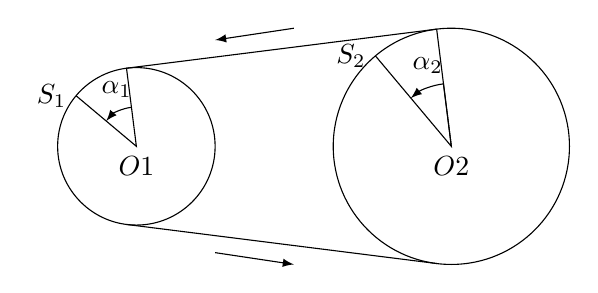
\begin{tikzpicture}[>=latex]
        \draw (0,0)node[below]{$O1$} circle (1);
        \draw (4,0)node[below]{$O2$} circle (1.5);
        \draw (140:1)node[left]{$S_1$}--(0,0)--(97.2:1)--+(7.18:3.97)--(4,0)
        --+(130:1.5)node[left]{$S_2$};    % --+表示以上一个点为(0,0)
        \draw (-97.2:1)--+(-7.18:3.97);
        \draw[->] (97.2:0.5) arc (97.2:140:0.5);
        \draw[->] (4,0)--+(97.2:0.8) arc (97.2:130:0.8);
        \node at (-0.25,0.5)[above]{$\alpha_1$};
        \node at (4-0.3,0.8)[above]{$\alpha_2$};
        \draw[<-] (1,1.35)--(2,1.5);
        \draw[->] (1,-1.35)--(2,-1.5);

    \end{tikzpicture}

    \caption{<caption>}
\end{figure}

\end{document}